\newcommand{\antOffx}{-0.4}
\newcommand{\antOffy}{ 0.3}

% Triangle:
\newcommand{\origin }{0.0}
\newcommand{\baseOffx }{6.5}
% (setq baseOffx '6.5)
% (setq tg '4.0)
% (* tg (sin (- (/ pi 2) (asin (/ tg baseOffx))))) 3.153
% (* tg (cos (- (/ pi 2) (asin (/ tg baseOffx))))) 2.461
\newcommand{\sinTheta }{3.153}
\newcommand{\cosTheta }{2.461}

% Parallel lines:
% (* (sqrt (- (* baseOffx baseOffx) (* tg tg))) (cos (asin (/ tg baseOffx)))) 4.038
\newcommand{\parrOff }{4.038}

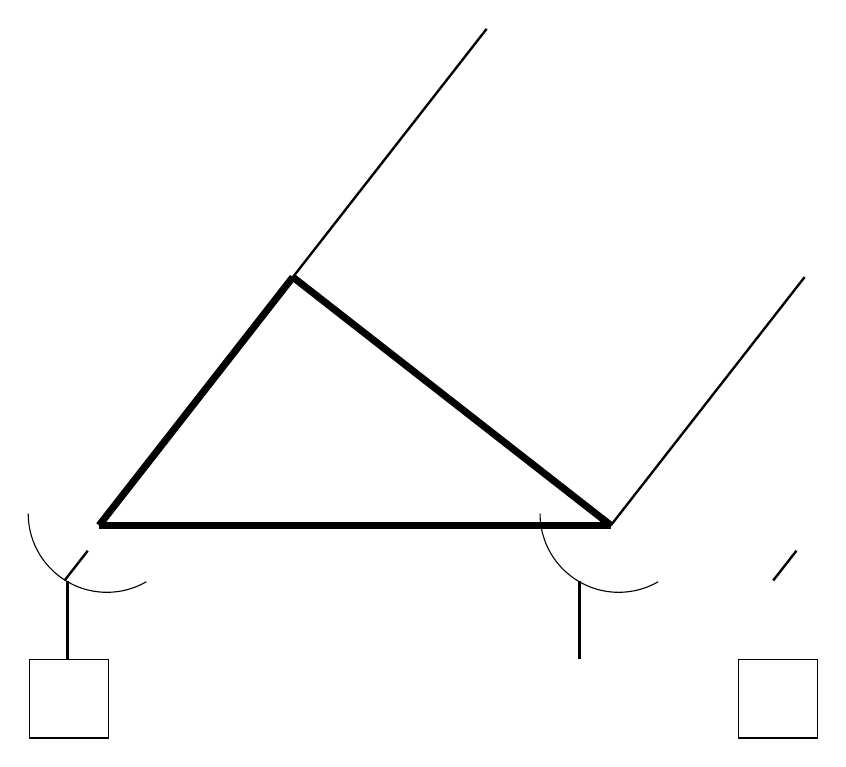
\begin{tikzpicture}

  % Parallel lines:
  \draw[line width= 0.3mm, black] (\cosTheta *2,           \sinTheta *2) -- (\cosTheta ,           \sinTheta );
  \draw[line width= 0.3mm, black] (\cosTheta *2+\parrOff , \sinTheta   ) -- (\cosTheta + \parrOff, \origin   );

  % Triangle:
  \draw[line width= 0.9mm, black] (\baseOffx, \origin   ) -- (\cosTheta , \sinTheta );
  \draw[line width= 0.9mm, black] (\cosTheta, \sinTheta ) -- (\origin   , \origin   );
  \draw[line width= 0.9mm, black] (\baseOffx, \origin   ) -- (\origin   , \origin   );

  % Telescopes:
    % Dish:
    \draw ( \origin   -0.5+\antOffx, \origin -0.15+\antOffy ) arc (180:300:1cm);
    \draw ( \baseOffx -0.5+\antOffx, \origin -0.15+\antOffy ) arc (180:300:1cm);
    % Pedestal:
    \draw[line width= 0.3mm, black] (\baseOffx +\antOffx , -2.0+\antOffy ) -- (\baseOffx +\antOffx , -1.0+\antOffy );
    \draw[line width= 0.3mm, black] (0.0+\antOffx , -2.0+\antOffy ) -- (0.0+\antOffx , -1.0+\antOffy );
    % Feed:
    \draw[line width= 0.3mm, black] (\antOffx+\cosTheta*1.12-2.5,   \sinTheta*1.12-\sinTheta-1+\antOffy) -- (\antOffx+\cosTheta-2.5,   \sinTheta-\sinTheta-1+\antOffy);
    \draw[line width= 0.3mm, black] (\antOffx+\cosTheta*1.12-2.5+9, \sinTheta*1.12-\sinTheta-1+\antOffy) -- (\antOffx+\cosTheta-2.5+9, \sinTheta-\sinTheta-1+\antOffy);

  % Correlator
  \draw [black] (-2.5+1.62,-2.7) rectangle (-1.5+1.62, -1.7);
  \draw [black] (-2.5+1.62+9,-2.7) rectangle (-1.5+1.62+9, -1.7);

\end{tikzpicture}

%%% Local Variables:
%%% mode: latex
%%% TeX-master: "../Lecture"
%%% End: